%%%%%%%%%%%%%%%%%%%%%%%%%%%%%%%%%%%%%%%%%
% Short Sectioned Assignment
% LaTeX Template
% Version 1.0 (5/5/12)
%
% This template has been downloaded from:
% http://www.LaTeXTemplates.com
%
% Original author:
% Frits Wenneker (http://www.howtotex.com)
%
% License:
% CC BY-NC-SA 3.0 (http://creativecommons.org/licenses/by-nc-sa/3.0/)
%
%%%%%%%%%%%%%%%%%%%%%%%%%%%%%%%%%%%%%%%%%

%----------------------------------------------------------------------------------------
%	PACKAGES AND OTHER DOCUMENT CONFIGURATIONS
%----------------------------------------------------------------------------------------

\documentclass[paper=a4, fontsize=12pt]{scrartcl} % A4 paper and 11pt font size

\usepackage[utf8]{vietnam}
\usepackage[vietnamese]{babel}

% \usepackage[T1]{fontenc} % Use 8-bit encoding that has 256 glyphs
% \usepackage{fourier} % Use the Adobe Utopia font for the document - comment this line to return to the LaTeX default
% \usepackage[english]{babel} % English language/hyphenation
\usepackage{amsmath,amsfonts,amsthm,amssymb} % Math packages

\usepackage{lipsum} % Used for inserting dummy 'Lorem ipsum' text into the template

\usepackage{sectsty} % Allows customizing section commands
% \allsectionsfont{\centering \normalfont\scshape} % Make all sections centered, the default font and small caps

\usepackage{enumitem}

\usepackage{fancyhdr} % Custom headers and footers
\pagestyle{fancyplain} % Makes all pages in the document conform to the custom headers and footers
\fancyhead{} % No page header - if you want one, create it in the same way as the footers below
\fancyfoot[L]{} % Empty left footer
\fancyfoot[C]{} % Empty center footer
\fancyfoot[R]{\thepage} % Page numbering for right footer
\renewcommand{\headrulewidth}{0pt} % Remove header underlines
\renewcommand{\footrulewidth}{0pt} % Remove footer underlines
\setlength{\headheight}{13.6pt} % Customize the height of the header
\numberwithin{equation}{section} % Number equations within sections (i.e. 1.1, 1.2, 2.1, 2.2 instead of 1, 2, 3, 4)
\numberwithin{figure}{section} % Number figures within sections (i.e. 1.1, 1.2, 2.1, 2.2 instead of 1, 2, 3, 4)
\numberwithin{table}{section} % Number tables within sections (i.e. 1.1, 1.2, 2.1, 2.2 instead of 1, 2, 3, 4)

\setlength\parindent{0pt} % Removes all indentation from paragraphs - comment this line for an assignment with lots of text

\newenvironment{theorem}[2][Định lý]{\begin{trivlist}
\item[\hskip \labelsep {\bfseries #1}\hskip \labelsep {\bfseries #2.}]}{\end{trivlist}}
\newenvironment{lemma}[2][Bổ đề]{\begin{trivlist}
\item[\hskip \labelsep {\bfseries #1}\hskip \labelsep {\bfseries #2.}]}{\end{trivlist}}
\newenvironment{exercise}[2][Bài tập]{\begin{trivlist}
\item[\hskip \labelsep {\bfseries #1}\hskip \labelsep {\bfseries #2.}]}{\end{trivlist}}
\newenvironment{reflection}[2][Reflection]{\begin{trivlist}
\item[\hskip \labelsep {\bfseries #1}\hskip \labelsep {\bfseries #2.}]}{\end{trivlist}}
\newenvironment{proposition}[2][Mệnh đề]{\begin{trivlist}
\item[\hskip \labelsep {\bfseries #1}\hskip \labelsep {\bfseries #2.}]}{\end{trivlist}}
\newenvironment{corollary}[2][Hệ quả]{\begin{trivlist}
\item[\hskip \labelsep {\bfseries #1}\hskip \labelsep {\bfseries #2.}]}{\end{trivlist}}
\newenvironment{solution}[2][Lời giải]{\begin{trivlist}
\item[\hskip \labelsep {\bfseries #1}\hskip\labelsep{}]}{\end{trivlist}}
\newenvironment{way}[2][Cách]{\begin{trivlist}
\item[\hskip \labelsep {\bfseries #1}\hskip \labelsep {\bfseries #2.}]}{\end{trivlist}}

\newcommand{\N}{\mathbb{N}}
\newcommand{\Z}{\mathbb{Z}}
\newcommand{\R}{\mathbb{R}}
\newcommand{\F}{\mathbb{F}}

\usepackage{setspace}
\usepackage{graphicx}
\onehalfspacing % Set line spacing to 1.5
%----------------------------------------------------------------------------------------
%	TITLE SECTION
%----------------------------------------------------------------------------------------

\newcommand{\horrule}[1]{\rule{\linewidth}{#1}} % Create horizontal rule command with 1 argument of height
\newcommand{\argmax}{\arg\!\max}
\title{	
\normalfont \normalsize 
\textsc{ĐẠI HỌC QUỐC GIA TP.HCM \\ TRƯỜNG ĐẠI HỌC KHOA HỌC TỰ NHIÊN \\ KHOA TOÁN - TIN HỌC} \\ [25pt] % Your university, school and/or department name(s)
\horrule{0.5pt} \\[0.4cm] % Thin top horizontal rule
\huge QUY HOẠCH PHI TUYẾN \\ BÀI TẬP CUỐI KỲ \\ % The assignment title
\horrule{2pt} \\[0.5cm] % Thick bottom horizontal rule
}

\author{Lê Nhựt Nam} % Your name

\date{\normalsize\today} % Today's date or a custom date

\begin{document}

\maketitle % Print the title

    \section{Bài 01}


\begin{corollary}{1}
    \label{coro:slater}
    Giả sử các hàm $\{g_i \}_1^r$ là lồi, và hàm $\{h_j \}_1^r$ là các hàm affine. Gọi $x^*$ là một cực tiểu địa phương của bài toán $(P)$. Nếu tồn tại một điểm khả thi $x_0$, khả thi ngặt cho ràng buộc động (active constraints) $g_i$ là 
    \begin{equation}
        g_i(x_0) < 0, i \in I(x^*)
    \end{equation}
    thì các điều kiện KKT là thỏa mãn tại $x^*$
\end{corollary}

Bài toán. Tìm giá trị cực tiểu của hàm 
\begin{equation}
    f(x, y) = (x-2)^2 + (y-1)^2
\end{equation}
thỏa mãn điều kiện $y \geq x^2$ và $x + y \leq 2$

\begin{solution}{*}
    Bài toán tối ưu có thể được viết như sau:
    \begin{equation}
        \begin{aligned}
            \min \quad & (x-2)^2 + (y-1)^2\\
            \textrm{s.t.} \quad & x + y - 2 \leq 0\\
              & x^2 - y \leq 0    \\
        \end{aligned}
    \end{equation}
    Các thành phần trong bài toán này như sau:
    \begin{align}
        \begin{aligned}
            f(x,y) &= (x-2)^2 + (y-1)^2\\
            g_1(x,y) &= x + y - 2\\
            g_2(x, y) &= x^2 - y 
        \end{aligned}
    \end{align}
    
    Ta thấy miền ràng buộc (constraint region) là compact. Bởi vì các ràng buộc là những hàm lồi (convex function), nên tồn tại một lời giải khả thi nghiêm ngặt, điều kiện Slater (Hệ quả \ref{coro:slater}) thỏa mãn. Điều này dẫn đến việc các điều kiện KKT phải thỏa mãn tại bất kỳ cực tiểu địa phương nào. Do đó, ta có hàm Lagrangian như sau:
    \begin{align}
        \begin{aligned}
            L(x, y, \lambda) &= f(x, y) + \lambda_1g_1(x,y) + \lambda_2g_2(x,y)\\
            L(x, y, \lambda) &= (x-2)^2 + (y-1)^2 + \lambda_1(x + y - 2) + \lambda_2(x^2 - y)
        \end{aligned}
    \end{align}
    và các điều kiện KKT 
    \begin{enumerate}[label=(\alph*)]
        \item \begin{equation}
            \frac{\partial L}{\partial x} = 2(x - 2) + \lambda_1 + 2x\lambda_2 = 0,
        \end{equation}
        \item \begin{equation}
            \frac{\partial L}{\partial y} = 2(y-1) + \lambda_1 - \lambda_2 = 0,
        \end{equation}
        \item \begin{equation}
            \lambda_1 \geq 0, x + y - 2 \leq 0, \lambda_1(x + y - 2) = 0,
        \end{equation}
        \item \begin{equation}
            \lambda_2 \geq 0, x^2 - y \leq 0, \lambda_2(x^2 - y) = 0
        \end{equation}
    \end{enumerate}
    Đơn giản biểu thức (a), và (b), ta thu được
    \begin{equation}
        x = \dfrac{4-\lambda_1}{2(\lambda_2 + 1)};\quad y = \dfrac{\lambda_2 - \lambda_1 + 2}{2}
    \end{equation}
    Ta xem xét các trường hợp
    \begin{enumerate}[label=(\roman*)]
        \item $\lambda_1 > 0$ và $\lambda_2 > 0$. Ta có hệ phương trình:
        \begin{equation}
            \begin{cases}
                x + y - 2 = 0\\
                x^2 - y = 0\\
            \end{cases}
        \end{equation}
        Giải hệ này, ta được nghiệm  $(x_1, y_1) = (1, 1)$ và $(x_2, y_2) = (-2, 4)$. 
        \begin{itemize}
            \item Trường hợp 1: $(x_1, y_1) = (1, 1)$, ta có 
            \begin{equation}
                \begin{cases}
                    \dfrac{4-\lambda_1}{2(\lambda_2 + 1)} = 1 \Leftrightarrow \lambda_1 + 2\lambda_2 = 2\\\\
                    \dfrac{\lambda_2 - \lambda_1 + 2}{2} = 1 \Leftrightarrow -\lambda_1 + \lambda_2 = 0
                \end{cases}
                \Leftrightarrow \begin{cases}
                    \lambda_1 = \dfrac{2}{3}\\\\
                    \lambda_2 = \dfrac{2}{3}
                \end{cases}
            \end{equation}
            \item Trường hợp 2: $(x_2, y_2) = (-2, 4)$, ta có:
            \begin{equation}
                \begin{cases}
                    \dfrac{4-\lambda_1}{2(\lambda_2 + 1)} = -2 \Leftrightarrow \lambda_1  -4\lambda_2 = 8\\\\
                    \dfrac{\lambda_2 - \lambda_1 + 2}{2} = 4 \Leftrightarrow -\lambda_1 + \lambda_2 = 6
                \end{cases}
                \Leftrightarrow \begin{cases}
                    \lambda_1 = \dfrac{-32}{3}\\\\
                    \lambda_2 = \dfrac{-14}{3}
                \end{cases}
            \end{equation}
        \end{itemize}
        Ta loại điểm $(x_2, y_2) = (-2, 4)$ vì nó tương ứng với các nhân tử không thỏa mãn trường hợp đang xét. Do đó, điểm $(1,1)$ là một điểm KKT tương ứng với các nhân tử $(\lambda_1, \lambda_2) = \left(\dfrac{2}{3},\dfrac{2}{3}\right)$ và nó cũng thỏa mãn các ràng buộc đầu bài.
        \item $\lambda_1 > 0$ và $\lambda_2 = 0$. Từ điều kiện $(c)$ và biểu thức (1.10), ta có:
        \begin{equation}
            \begin{cases}
                x + y - 2 = 0 \\
                x = \dfrac{4-\lambda_1}{2}\\\\
                y = \dfrac{- \lambda_1 + 2}{2}
            \end{cases}
            \Leftrightarrow \lambda_1 = 1
        \end{equation}
        Do đó, điểm $\left(\dfrac{3}{2},\dfrac{1}{2}\right)$ là một điểm tương ứng với các nhân tử $(\lambda_1, \lambda_2) = (1, 0)$. Tuy nhiên điểm này không thỏa mãn ràng buộc, do đó nó không phải điểm KKT.
        \item $\lambda_1 = 0$ và $\lambda_2 > 0$. Ta có:
        \begin{equation}
            \begin{cases}
                x^2 - y = 0\\
                x = \dfrac{4}{2(\lambda_2 + 1)}\\\\
                y = \dfrac{\lambda_2 + 2}{2}
            \end{cases}
            \Leftrightarrow 
            \begin{cases}
                \left( \dfrac{4}{2(\lambda_2 + 1)}\right)^2 - \dfrac{\lambda_2 + 2}{2} = 0\\\\
                x = \dfrac{4}{2(\lambda_2 + 1)}\\\\
                y = \dfrac{\lambda_2 + 2}{2}
            \end{cases}
            \Leftrightarrow 
            \begin{cases}
                \lambda_2 \approx 0.71618\\
                x \approx 1.16538 \\
                y \approx 1.35803
            \end{cases}
        \end{equation}
        Hai điểm này không thỏa mãn ràng buộc của bài toán.
        \item $\lambda_1 = 0$ và $\lambda_2 = 0$. Từ biểu thức (1.10), ta được $(x, y) = (2, 1)$ tuy nhiên điểm này lại không thỏa mãn các ràng buộc đầu bài.
    \end{enumerate}
    Giá trị hàm mục tiêu tại các điểm mục tiêu:
    \begin{itemize}
        \item $f(1,1) = 1$
    \end{itemize}
    Vậy cực tiểu của bài toán đạt tại điểm điểm $(x, y) = (1,1)$
\end{solution}
    \section{Bài 02}

Cho bài toán tối ưu
\begin{equation}
    \begin{aligned}
        \min \quad & -xy\\
        \textrm{s.t.} \quad & x + y = 8\\
          &x\geq0, y \geq 0    \\
    \end{aligned}
\end{equation}
mô hình cho vấn đề tìm kiếm một hình chữ nhật có diện tích lớp nhất với chu vi 16.

\begin{enumerate}[label=(\alph*)]
\item Viết điều kiện FJ, và chứng minh rằng $\lambda_0 \ne 0$, và do đó điều kiện KKT được thỏa mãn tại tất cả các điểm mà thỏa điều kiện FJ.
\item Chứng minh rằng điểm $(x,y) = (4,4)$ thỏa mãn điều kiện KKT
\item Xác định tất cả các điểm KKT của bài toán.
\item Chứng minh rằng điểm $(x,y) = (4,4)$ thỏa mãn điều kiện đủ cấp hai, đó là một cực tiểu cục bộ (không nhất thiết là toàn cục) của bài toán. 
\end{enumerate}

\begin{solution}

    Các thành phần trong bài toán này như sau:
    \begin{align}
        \begin{aligned}
            f(x,y) &= -xy\\
            g_1(x,y) &= -x\\
            g_2(x, y) &= -y\\
            h_1(x,y) &= x + y - 8
        \end{aligned}
    \end{align}
    \begin{enumerate}
        \item Ta hình thành dạng yếu của hàm Lagrangian như sau:
    \begin{equation}
        L = -\lambda_0xy -\lambda_1x - \lambda_2y + \mu_1(x + y - 8)
    \end{equation}
    Các điều kiện Fritz John (FJ) được viết như sau:
    \begin{enumerate}[label=(\alph*)]
        \item \begin{equation}
            -\lambda_0y - \lambda_1 + \mu_1 = 0
        \end{equation}
        \item \begin{equation}
            -\lambda_0x - \lambda_2 + \mu_1 = 0
        \end{equation}
        \item \begin{equation}
            \lambda_1 \geq 0, - x \leq 0, \lambda_1x = 0
        \end{equation}
        \item \begin{equation}
            \lambda_2 \geq 0, - y \leq 0, \lambda_2y = 0
        \end{equation}
    \end{enumerate}
    Từ biểu thức (2.4) và (2.5), có:
    \begin{equation}
        x = \dfrac{-\lambda_2 + \mu_1}{\lambda_0},\quad y = \dfrac{-\lambda_1 + \mu_1}{\lambda_0}
    \end{equation}
    Dựa trên các điều kiện này, $\lambda_0 \ne 0$. Nếu $\lambda_0 = 0$, thì điều kiện $(a)$, và $(b)$ lần lượt trở thành:
    \begin{equation}
        \begin{cases}
            - \lambda_1 + \mu_1 = 0 \\ 
            - \lambda_2 + \mu_1 = 0
        \end{cases}
        \Leftrightarrow \mu_1 =  \lambda_1 = \lambda_2
    \end{equation}
    Ta sẽ không xác định được $x, y$ trong trường hợp này. Do đó, điều này là không thể. Do đó điều kiện KKT được thỏa mãn tại tất cả các điểm mà thỏa điều kiện FJ.
    \item Chứng minh rằng điểm $(x,y) = (4,4)$ thỏa mãn điều kiện KKT. Thay điểm $(x,y) = (4,4)$ vào các điều kiện FJ ở trên, ta được:
    \begin{enumerate}[label=(\alph*)]
        \item \begin{equation}
            -4\lambda_0 - \lambda_1 + \mu_1 = 0 \Leftrightarrow \lambda_0 = -\frac{-\lambda_1+\mu_1}{4}
        \end{equation}
        \item \begin{equation}
            -4\lambda_0 - \lambda_2 + \mu_1 = 0 \Leftrightarrow \lambda_0 = -\frac{-\lambda_2+\mu_1}{4}
        \end{equation}
        \item \begin{equation}
            \lambda_1 \geq 0, - 4 \leq 0, 4\lambda_1 = 0
        \end{equation}
        \item \begin{equation}
            \lambda_2 \geq 0, - 4 \leq 0, 4\lambda_2 = 0
        \end{equation}
    \end{enumerate}
    Từ các biểu thức trên $\lambda_1 = \lambda_2 = 0$. Và từ biểu thức (2.8)
    \begin{equation}
        x = y =4
    \end{equation}
    Vậy, $(x,y) = (4,4)$ thỏa mãn điều kiện KKT.
    \item Xác định tất cả các điểm KKT của bài toán. Do bài toán đặt ra ban đầu là về tìm kiếm một hình chữ nhật có diện tích với chu vi là 16 nên $x, y$ phải khác 0, và từ biểu thức (2.8) ta có được:
    \begin{equation}
        x = \dfrac{\mu_1}{\lambda_0},\quad y = \dfrac{\mu_1}{\lambda_0}, \quad \lambda_1 = \lambda_2 = 0
    \end{equation}
    Do $x + y = 8$, nên
    \begin{equation}
        \dfrac{\mu_1}{\lambda_0} + \dfrac{\mu_1}{\lambda_0} = 8 \Leftrightarrow \mu_1 = 4\lambda_0 \Leftrightarrow x = y = 4
    \end{equation}
    Vậy, điểm $(x,y) = (4,4)$ là điểm KKT duy nhất của bài toán.
    \item \textbf{Đây là câu về điều kiện cấp hai.}
    \end{enumerate}
\end{solution}
    \section{Bài 03}

Xem xét bài toán
\begin{equation}
    \label{problem:03}
    \begin{aligned}
        \max \quad & x^2 + (y+1)^2\\
        \textrm{s.t.} \quad & -x^2 + y \geq 0\\
          &x + y \leq 2   \\
    \end{aligned}
\end{equation}
\begin{enumerate}[label=(\alph*)]
    \item Viết điều kiện FJ, và lập luận rằng $\lambda_0 \ne 0$
    \item Vẽ miền khả thi (feasible region), và bằng hình vẽ, xác định (các) lời giải tối ưu.
    \item Xác định tất cả các điểm mà thỏa mãn các điều kiện KKT; sau đó xác định các cực đại (toàn cục) giữa chứng.
\end{enumerate}


\begin{solution}

    Dựa trên nguyên lý đối ngẫu, ta viết lại bài toán như sau:
    \begin{equation}
        \begin{aligned}
            \min \quad & -x^2 - (y+1)^2\\
            \textrm{s.t.} \quad & x^2 - y \leq 0\\
              &x + y - 2\leq 0   \\
        \end{aligned}
    \end{equation}
    Các thành phần trong bài toán này như sau:
    \begin{align}
        \begin{aligned}
            f(x,y) &= -x^2 - (y+1)^2\\
            g_1(x,y) &= x^2 - y\\
            g_2(x, y) &= x + y - 2\\
        \end{aligned}
    \end{align}
    \begin{enumerate}[label=(\alph*)]
        \item Ta hình thành dạng yếu của hàm Lagrangian như sau:
        \begin{equation}
            L = -\lambda_0\left[x^2 + (y+1)^2\right] + \lambda_1(x^2 - y) + \lambda_2(x+y-2)
        \end{equation}
        Các điều kiện Fritz John (FJ) được viết như sau:
        \begin{itemize}
            \item \begin{equation}
                -2x\lambda_0 +2x\lambda_1 + \lambda_2 = 0 \Leftrightarrow x = \dfrac{\lambda_2}{2(\lambda_0 - \lambda_1)}
            \end{equation}
            \item \begin{equation}
                -2\lambda_0(y+1) -\lambda_1 + \lambda_2 = 0 \Leftrightarrow y = \dfrac{-2\lambda_0 - \lambda_1 + \lambda_2}{2\lambda_0},
            \end{equation}
            \item \begin{equation}
                \lambda_1 \geq 0, x^2 - y \leq 0, \lambda_1 (x^2 - y) = 0,
            \end{equation}
            \item \begin{equation}
                \lambda_2 \geq 0, x + y - 2 \leq 0, \lambda_2(x + y - 2) = 0
            \end{equation}
        \end{itemize}
        Nếu $\lambda_0 = 0$ thì biểu thức (3.6) không xác định. Do đó, $\lambda_0 \ne 0$.
        \item Vẽ miền khả thi (feasible region), và bằng hình vẽ, xác định (các) lời giải tối ưu.
        \begin{figure}[h!]
            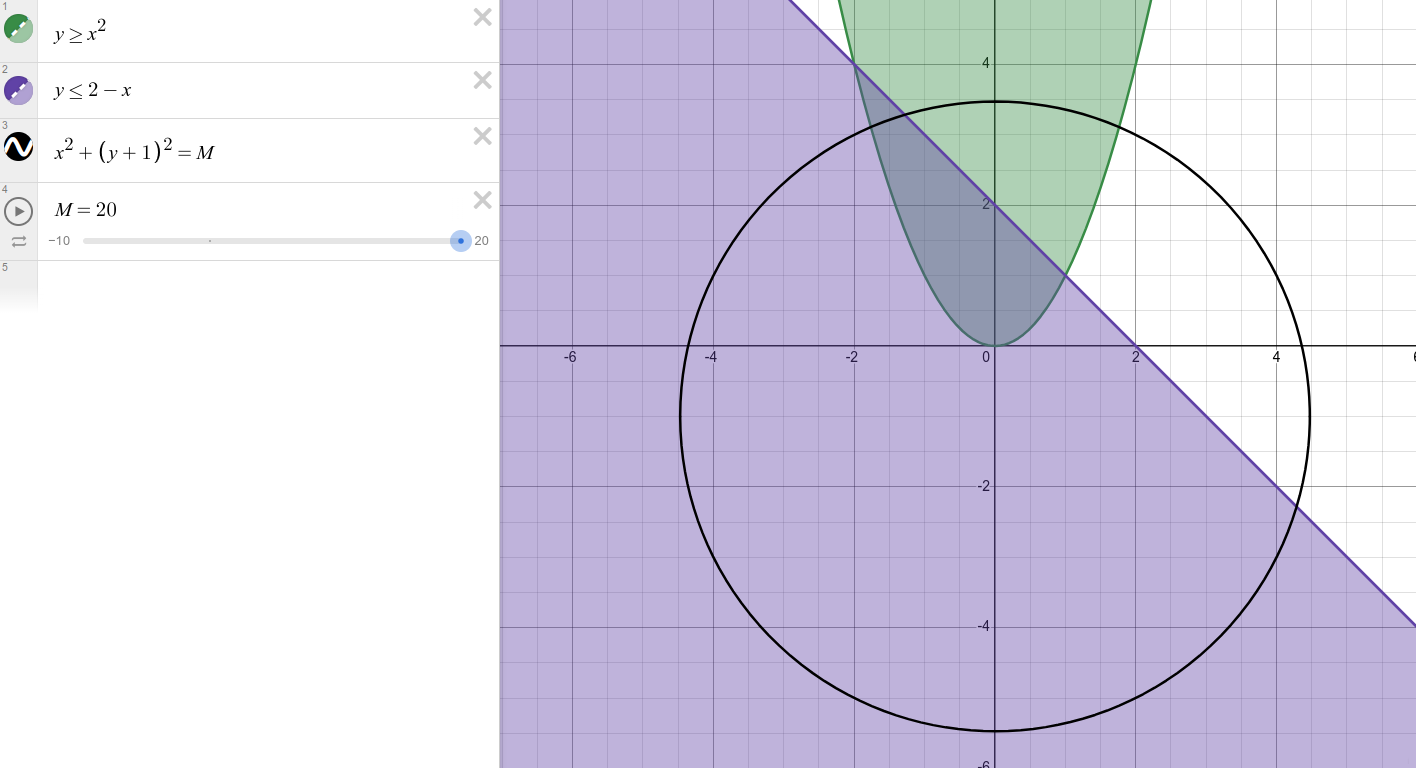
\includegraphics[width=0.85\linewidth]{figures/BT03.png}
            \caption{Miền khả thi của bài toán (\ref{problem:03}).}
            \label{fig:feasible_region_problem_03}
        \end{figure}
        \item Do $\lambda_ 0 \ne 0$, nên điều kiện KKT được thỏa mãn tại tất cả các điểm mà thỏa điều kiện FJ. Giả định rằng $\lambda_0 = 1$, ta có:
        \begin{equation}
            \begin{cases}
                x = \dfrac{\lambda_2}{2(1 - \lambda_1)} \\\\
                y = \dfrac{-2- \lambda_1 + \lambda_2}{2}
            \end{cases}
        \end{equation}
        Bằng cách kiểm tra các trường hợp
        \begin{enumerate}[label=(\roman*)]
            \item $\lambda_1 > 0$ và $\lambda_2 > 0$. Ta có hệ phương trình:
            \begin{equation}
                \begin{cases}
                    x^2 - y = 0 \\ 
                    x + y - 2 = 0
                \end{cases}
                \Leftrightarrow 
                \begin{cases}
                    x = 1 \\
                    y = 1
                \end{cases}
                \quad
                \text{hoặc}
                \quad
                \begin{cases}
                    x = -2 \\
                    y = 4
                \end{cases}
            \end{equation}
            Khi $(x, y) = (1, 1)$, ta giải được $(\lambda_1, \lambda_2) = \left(\dfrac{-2}{3}, \dfrac{10}{3}\right)$ nên điểm $(x, y) = (1, 1)$ không phải một điểm KKT. Và khi $(x, y) = (-2, 4)$, ta giải được $(\lambda_1, \lambda_2) = (14, 24)$ nên điểm $(x, y) = (-2, 4)$ là một điểm KKT.
            \item $\lambda_1 = 0$ và $\lambda_2 > 0$. Trong trường hợp này, thay $\lambda_1 = 0$, ta được:
            \begin{equation}
                \begin{cases}
                    x = \dfrac{\lambda_2}{2} \\\\
                    y = \dfrac{-2 + \lambda_2}{2}\\
                    x + y - 2 = 0
                \end{cases}
            \end{equation}
            Giải hệ này, ta được $\lambda_2 = 3$, $(x, y) = \left(\dfrac{3}{2}, \dfrac{1}{2}\right)$ là một điểm KKT.
            \item $\lambda_1 > 0$ và $\lambda_2 = 0$. Tương tự, ta thay $\lambda_2 = 0$, ta được:
            \begin{equation}
                \begin{cases}
                    x = 0 \\\\
                    y = \dfrac{-2- \lambda_1}{2}\\
                    y - 2 = 0
                \end{cases}
            \end{equation}
            Giải hệ này, ta được $\lambda_1 =- 6$, điểm $(x, y)$ trong trường hợp này không phải một điểm KKT.
            \item $\lambda_1 = 0$ và $\lambda_2 = 0$. Ta có được nghiệm $(x, y) = (0, -1)$
            là một điểm KKT.
        \end{enumerate}
        Các điểm KKT lần lượt là $(0, -1), (-2, 4), \left(\dfrac{3}{2}, \dfrac{1}{2}\right)$
    \end{enumerate}
\end{solution}

    \section{Bài 04}

Trong bài toán,
\begin{equation}
    \begin{aligned}
        \min \quad & \sum_{j=1}^n\frac{c_j}{x_j}\\
        \textrm{s.t.} \quad & \sum_{j=1}^na_jx_j = b,\\
          &x_j \geq 0, j = 1, \dots, n,  \\
    \end{aligned}
\end{equation}
trong đó $a_j, c_j, b$ là các hằng số dương. Viết điều kiện FJ, và nếu áp dụng điều kiện KKT. Sau đó giải (các) nghiệm tối ưu $x^{*} = (x^{*}_1, x^{*}_2, \dots, x^{*}_n)$.

\begin{solution}

    Các thành phần của bài toán
    \begin{equation}
        \begin{cases}
            f(x) = \sum_{j=1}^n\frac{c_j}{x_j} \\
            h_1(x) = \sum_{j=1}^na_jx_j - b
        \end{cases}
    \end{equation}
    Ta thử viết các điều kiện Fritz John. Bằng cách tính toán, ta hình thành dạng yếu của hàm Lagrangian như sau:
    \begin{equation}
        L = \lambda_0\left(\sum_{j=1}^n\frac{c_j}{x_j}\right) + \mu_1\left(\sum_{j=1}^na_jx_j - b\right)
    \end{equation}
    Và ta viết được các điều kiện FJ như sau:
    \begin{enumerate}[label=(\alph*)]
        \item \begin{equation}
            -\lambda_0\left(\sum_{j=1}^n\frac{c_j}{x^2_j}\right) + \mu_1\left(\sum_{j=1}^na_j\right) = 0
        \end{equation}
    \end{enumerate}
    Nếu $\lambda_0 = 0$, thì $\mu_1 = 0$, điều này dẫn đến bài toán vô nghĩa. Thế nên, $\lambda_0 \ne 0$. Ta sử dụng hàm Lagrangian và viết các điều kiện KKT để dễ dàng hơn trong việc giải quyết bài toán này. Ta có hàm Lagrangian như sau:
    \begin{equation}
        L(x, \lambda) = \sum_{j=1}^n\frac{c_j}{x_j} + \mu_1\left(\sum_{j=1}^na_jx_j - b\right)
    \end{equation}
    và các điều kiện KKT được viết như sau:
    \begin{enumerate}[label=(\alph*)]
        \item \begin{equation}
            \dfrac{\partial L}{\partial x_j} = -\left(\sum_{j=1}^n\frac{c_j}{x^2_j}\right) + \mu_1\left(\sum_{j=1}^na_j\right) = 0, 
        \end{equation}
        \item \begin{equation}
            \sum_{j=1}^na_jx_j - b = 0, 
        \end{equation}
    Tính tổng biểu thức (4.6), ta có:
    \begin{equation}
        -\left(\sum_{j=1}^nc_j\right)\left(\sum_{j=1}^nx^2_j\right)^{-1} + \mu_1\left(\sum_{j=1}^na_j\right) = -\mathbf{C}\mathbf{x}^{-1} + \mu_1\mathbf{A} = 0\Leftrightarrow \mathbf{x} = \dfrac{\mathbf{C}}{\mu_1\mathbf{A}}
    \end{equation}
    Và dựa trên biểu thức (4.7), ta có:
    \begin{equation}
        \sum_{j=1}^na_jx_j - b = \left(\sum_{j=1}^na_j\right)\left(\sum_{j=1}^nx_j\right) - b = \mathbf{A}\mathbf{x} - b = \mathbf{A}\dfrac{\mu_1\mathbf{A}}{\mathbf{C}} - b = 0
    \end{equation}
    Ta tính được:
    \begin{equation}
        \mu_1 = \dfrac{\mathbf{C}b}{\mathbf{A}^2}
    \end{equation}
    Suy ra được:
    \begin{equation}
        \mathbf{x} = \dfrac{\mathbf{A}}{b} \quad\text{hay}\quad b\mathbf{x} = \mathbf{A}
    \end{equation}
    Ta giải phương trình $b\mathbf{x} = \mathbf{A}$ thì thu được nghiệm tối ưu $x^{*} = (x^{*}_1, x^{*}_2, \dots, x^{*}_n)$.
    \end{enumerate}
\end{solution}
    \section{Bài 05}

Xem xét bài toán
\begin{equation}
    \begin{aligned}
        \min \quad & x^2 + y^2 + z^2\\
        \textrm{s.t.} \quad & xyz \geq 8\\
          & x \geq 0, y \geq 0, z \geq 0\\
    \end{aligned}
\end{equation}

\begin{enumerate}[label=(\alph*)]
    \item Tìm tất cả các điểm thỏa mãn điều kiện KKT.
    \item Sử dụng kiểm tra thỏa mãn bậc hai để xác định tất các các cực tiểu cục bộ và toàn cục.
\end{enumerate}

\begin{solution}

    Các thành phần trong bài toán này như sau:
    \begin{align}
        \begin{aligned}
            f(x,y) &= x^2 + y^2 + z^2\\
            g_1(x,y) &= - xyz - 8\\
            g_2(x, y) &= -x\\
            g_3(x, y) &= -y\\
            g_4(x, y) &= -z\\
        \end{aligned}
    \end{align}
    Ta viết hàm Lagrangian như sau:
    \begin{equation}
        L(x, y, z, \lambda) = (x^2 + y^2 + z^2) - \lambda_1(xyz + 8) - \lambda_2x - \lambda_3y - \lambda_4z
    \end{equation}
    và các điều kiện KKT được viết như sau:
    \begin{itemize}
        \item \begin{equation}
            \dfrac{\partial L}{\partial x} = 2x - \lambda_1yz - \lambda_2 = 0 \Leftrightarrow 2x^2 - \lambda_1xyz - \lambda_2x = 0
        \end{equation}
        \item \begin{equation}
            \dfrac{\partial L}{\partial y} = 2y - \lambda_1xz - \lambda_3 = 0 \Leftrightarrow 2y^2 - \lambda_1xyz - \lambda_3y = 0
        \end{equation}
        \item \begin{equation}
            \dfrac{\partial L}{\partial z} = 2z - \lambda_1xy - \lambda_4 = 0 \Leftrightarrow 2z^2 - \lambda_1xyz - \lambda_4z = 0
        \end{equation}
        \item \begin{equation}
            \lambda_1 \geq 0, xyz - 8 \geq 0, \lambda_1(xyz - 8) = 0
        \end{equation}
        \item \begin{equation}
            \lambda_2 \geq 0, x \geq 0, \lambda_2x = 0
        \end{equation}
        \item \begin{equation}
            \lambda_3 \geq 0, y \geq 0, \lambda_3y = 0
        \end{equation}
        \item \begin{equation}
            \lambda_4 \geq 0, z \geq 0, \lambda_4z = 0
        \end{equation}
    \end{itemize}
    \begin{enumerate}[label=(\alph*)]
        \item Tìm tất cả các điểm thỏa mãn điều kiện KKT. Ta xem xét các trường hợp như sau:
        \begin{enumerate}[label=(\roman*)]
            \item TH1 ($\lambda_1 > 0$). Từ biểu thức (5.7), ta có: $xyz = 8$, từ các biểu thức (5.4), (5.5), và (5.6) thu được hệ phương trình
            \begin{equation}
                \begin{cases}
                    x(2x - \lambda_2) = 8\lambda_1\\
                    y(2y - \lambda_3) = 8\lambda_1\\
                    z(2z - \lambda_4) = 8\lambda_1\\
                \end{cases}
            \end{equation}
            Ta có thể chứng minh được $x, y, z >0$. Và điều này dẫn tới việc $\lambda_2, \lambda_3, \lambda_4$ đều bằng 0. Ta viết lại hệ trên:
            \begin{equation}
                \begin{cases}
                    2x^2 = 8\lambda_1 \Leftrightarrow x = 2\sqrt{2\lambda_1}\\
                    2y^2 = 8\lambda_1 \Leftrightarrow y = 2\sqrt{2\lambda_1}\\
                    2z^2 = 8\lambda_1 \Leftrightarrow z = 2\sqrt{2\lambda_1}\\
                \end{cases}
            \end{equation}
            Ta có: $xyz = 8 \Leftrightarrow \left(2\sqrt{2\lambda_1}\right)^3 = 8 \Leftrightarrow \lambda_1 = \dfrac{1}{2}$.
            Vậy, $ x = y = z = 2$
            \item TH2 ($\lambda_1 = 0$). Trường hợp này, $x,y,z$ suy biến về 0. Ta không tìm được điểm KKT nào.
        \end{enumerate}
        \item Sử dụng kiểm tra thỏa mãn bậc hai để xác định tất các các cực tiểu cục bộ và toàn cục. \textbf{Đây là câu về điều kiện cấp hai.}
    \end{enumerate}
\end{solution}
    \section{Bài 06}

Xemx xét bài toán 
\begin{equation}
    \begin{aligned}
        \min \quad & \ln x - y\\
        \textrm{s.t.} \quad & x^2 + y^2 \leq 4\\
          & x \geq 1\\
    \end{aligned}
\end{equation}

\begin{enumerate}[label=(\alph*)]
    \item Tìm tất cả các điểm thỏa mãn điều kiện FJ.
    \item Tìm tất cả các điểm thỏa mãn điều kiện KKT.
    \item Những điểm KKT nào mà có giá trị mục tiêu thấp nhất (lowest objective value)?
    \item Xác định liệu một thỏa mãn điều kiện đủ cấp hai được thỏa mãn tại mỗi điểm KKT.
\end{enumerate}

\begin{solution}

    Các thành phần trong bài toán này như sau:
    \begin{align}
        \begin{aligned}
            f(x,y) &= \ln x - y\\
            g_1(x,y) &= x^2 + y^2 - 4\\
            g_2(x, y) &= -x + 1\\
        \end{aligned}
    \end{align}

    \begin{enumerate}[label=(\alph*)]
        \item Tìm tất cả các điểm thỏa mãn điều kiện FJ. 

        Ta hình thành dạng yếu của hàm Lagrangian như sau:
        \begin{equation}
            L(x, y, \lambda) = \lambda_0(\ln x - y) + \lambda_1(x^2 + y^2 - 4) - \lambda_2(x + 1)
        \end{equation}
        và các điều kiện FJ
        \begin{itemize}
            \item \begin{equation}
                \dfrac{\lambda_0}{x} + 2x\lambda_1 - \lambda_2 = 0
            \end{equation}
            \item \begin{equation}
                -\lambda_0 + 2y\lambda_1 = 0
            \end{equation}
            \item \begin{equation}
                \lambda_1 \geq 0, x^2 + y^2 - 4 \leq 0, \lambda_1(x^2 + y^2 - 4) = 0
            \end{equation}
            \item \begin{equation}
                \lambda_2 \geq 0, -x + 1 \leq 0, -\lambda_2(x-1) = 0
            \end{equation}
        \end{itemize}
        Giả sử $\lambda_0 = 0$, ta có:
        \begin{equation}
            \begin{cases}
                2x\lambda_1 - \lambda_2 = 0 \Leftrightarrow x = \dfrac{\lambda_2}{2\lambda_1}\\
                2y\lambda_1 = 0\\
            \end{cases}
        \end{equation}
        Điều này cho thấy $\lambda_1$ không thể bằng 0. Do đó, $y$ phải bằng 0. Thay $x$ vào biểu thức (6.7), ta tính được $\lambda_2 = 0$ hoặc $\lambda_2 = 2\lambda_1$. Trong cả trường hợp hai, ta được $x = 1$. Vậy điểm $(x, y) = (1, 0)$ là một điểm thỏa mãn điều kiện FJ. 
        
        Giả sử $\lambda_0 \ne 0$. Ta xét từng trường hợp dấu của các nhân tử
        \begin{itemize}
            \item TH1 ($\lambda_1 > 0, \lambda_2 > 0$): Từ biểu thức (6.6) và (6.7) ta có hệ 
            \begin{equation}
                \begin{cases}
                    x^2 + y^2 - 4 = 0\\
                    x - 1 = 0\\
                \end{cases}
                \Leftrightarrow 
                \begin{cases}
                    x = 1\\
                    y = \pm \sqrt{3}
                \end{cases}
            \end{equation}
            Các điểm $(x, y) = (1, \sqrt{3})$ và $(x, y) = (1, -\sqrt{3})$ thỏa mãn điều kiện FJ.
            \item TH2 ($\lambda_1 = 0, \lambda_2 = 0$): Từ biểu thức (6.4) và (6.5) ta có:
            \begin{equation}
                \begin{cases}
                    \dfrac{\lambda_0}{x} = 0\\
                    -\lambda_0 = 0
                \end{cases}
            \end{equation}
            Trường hợp này vi phạm điều kiện $\lambda_0 \ne 0$.
            \item TH3 ($\lambda_1 > 0, \lambda_2 = 0$). Từ biểu thức (6.4), (6.5), và (6.6), ta có
            \begin{equation}
                \begin{cases}
                    x^2 + y^2 = 4\\ 
                    y = \dfrac{\lambda_0}{2\lambda_1}\\
                    x = -\dfrac{\lambda_0}{2\lambda_1}\\
                \end{cases}
            \end{equation}
            Giải hệ này, ta được nghiệm $(x, y) = (\sqrt{2}, -\sqrt{2})$ thỏa mãn.
            \item TH4 ($\lambda_1 = 0, \lambda_2 > 0$). Từ biểu thức (6.5), $\lambda_1$ không thể bằng 0. Do đó, ta không tìm được điểm nào thỏa mãn FJ trong trường hợp này.
        \end{itemize}
        Vậy, các điểm thỏa mãn điều kiện FJ là $(x, y) = (\sqrt{2}, -\sqrt{2})$, $(x, y) = (1, 0)$, $(x, y) = (1, \sqrt{3})$ và $(x, y) = (1, -\sqrt{3})$.
        \item Tìm tất cả các điểm thỏa mãn điều kiện KKT.
        Ta hình thành hàm Lagrangian như sau:
        \begin{equation}
            L(x, y, \lambda) = (\ln x - y) + \lambda_1(x^2 + y^2 - 4) - \lambda_2(x + 1)
        \end{equation}
        và các điều kiện FJ
        \begin{itemize}
            \item \begin{equation}
                \dfrac{\partial L}{\partial x} = \dfrac{1}{x} + 2\lambda_1x - \lambda_2 = 0 
            \end{equation}
            \item \begin{equation}
                \dfrac{\partial L}{\partial y} = -1 + 2\lambda_1y = 0 \Leftrightarrow y = \dfrac{1}{2\lambda_1}
            \end{equation}
            \item \begin{equation}
                \lambda_1 \geq 0, x^2 + y^2 - 4 \leq 0, \lambda_1(x^2 + y^2 - 4) = 0
            \end{equation}
            \item \begin{equation}
                \lambda_2 \geq 0, -x + 1 \leq 0, -\lambda_2(x-1) = 0
            \end{equation}
        \end{itemize}
        Ta xét từng trường hợp dấu của các nhân tử
        \begin{itemize}
            \item TH1 ($\lambda_1 > 0, \lambda_2 > 0$). Từ biểu thức (6.15), và (6.16) ta có hệ
            \begin{equation}
                \begin{cases}
                    x^2 + y^2 = 4\\
                    x = 1
                \end{cases}
                \Leftrightarrow 
                \begin{cases}
                    x = 1\\
                    y = \pm\sqrt{3}
                \end{cases}
            \end{equation}
            Các điểm $(x, y) = (1, \sqrt{3})$ và $(x, y) = (1, -\sqrt{3})$ thỏa mãn điều kiện KKT.
            \item TH2 ($\lambda_1 = 0, \lambda_2 = 0$)
            Từ biểu thức (6.13) và (6.14) ta có:
            \begin{equation}
                \begin{cases}
                    \dfrac{1}{x} = 0\\
                    -1 = 0
                \end{cases}
            \end{equation}
            Hệ này vô lý nên không tìm được điểm nào thỏa mãn điều kiện KKT.
            \item TH3 ($\lambda_1 > 0, \lambda_2 = 0$). Từ biểu thức (6.13), (6.14), và (6.15), ta có
            \begin{equation}
                \begin{cases}
                    x^2 + y^2 = 4\\ 
                    y = \dfrac{1}{2\lambda_1}\\
                    x = -\dfrac{1}{2\lambda_1}\\
                \end{cases}
            \end{equation}
            Giải này ta thu được $\lambda_1 = \dfrac{\sqrt{2}}{4}$. Ta có điểm $(x, y) = (\sqrt{2}, -\sqrt{2})$ thỏa mãn điều kiện KKT.
            \item TH4 ($\lambda_1 = 0, \lambda_2 > 0$). Từ biểu thức (6.14), ta không thể tính được khi $\lambda_1 = 0$, nên ta không tìm được điểm nào thỏa mãn điều kiện KKT trong trường hợp này.
        \end{itemize}
        Vậy, các điểm $(x, y) = (\sqrt{2}, -\sqrt{2})$, $(x, y) = (1, \sqrt{3})$ và $(x, y) = (1, -\sqrt{3})$ là điểm thỏa mãn điều kiện KKT.
        \item Những điểm KKT nào mà có giá trị mục tiêu thấp nhất (lowest objective value)? Ta có giá trị hàm mục tiêu tại các điểm KKT như sau:
        \begin{itemize}
            \item $f(\sqrt{2}, -\sqrt{2}) = 1.7608$
            \item $f(1, -\sqrt{3}) = -\sqrt{3}$
            \item $f(1, -\sqrt{3}) = \sqrt{3}$
        \end{itemize}
        Vậy tại điểm $(x,y) = (1, -\sqrt{3})$ giá trị mục tiêu thấp nhất (lowest objective value).
        \item Xác định liệu một thỏa mãn điều kiện đủ cấp hai được thỏa mãn tại mỗi điểm KKT. \textbf{Đây là câu về điều kiện cấp hai.}
    \end{enumerate}
\end{solution}
    \section{Bài 07}

(Absence of KKT points) Xem xét bài toán
\begin{equation}
    \label{problem:07}
    \begin{aligned}
        \min \quad & x^2 + y^2\\
        \textrm{s.t.} \quad & x^2 - (y - 1)^3 = 0\\
    \end{aligned}
\end{equation}

\begin{enumerate}[label=(\alph*)]
    \item Giải bài toán này theo phương pháp hình học.
    \item Chứng minh rằng không tồn tại điểm nào thỏa mãn điều kiện KKT.
    \item Tìm tất cả các điểm thỏa mãn điều kiện FJ.
    \item Khi thử giải bài toán tối ưu bằng cách thế ngược $x^2 = (y - 1)^3$ trong hàm mục tiêu, do đó giảm thiểu nó về bài toán không ràng buộc:
    \begin{equation}
        \begin{aligned}
            \min \quad & y^2 + (y-1)^3\\
        \end{aligned}
    \end{equation}
    Những có điều gì đó chưa đúng với phương pháp này. Đó là gì, và làm thế nào để hiệu chỉnh lại cho đúng.
\end{enumerate}

\begin{solution}

    Các thành phần trong bài toán này như sau:
    \begin{align}
        \begin{aligned}
            f(x,y) &= x^2 + y^2\\
            h_1(x,y) &= x^2 - (y - 1)^3\\
        \end{aligned}
    \end{align}
    \begin{enumerate}[label=(\alph*)]
    \item Giải bài toán này theo phương pháp hình học.
    \begin{figure}[h!]
        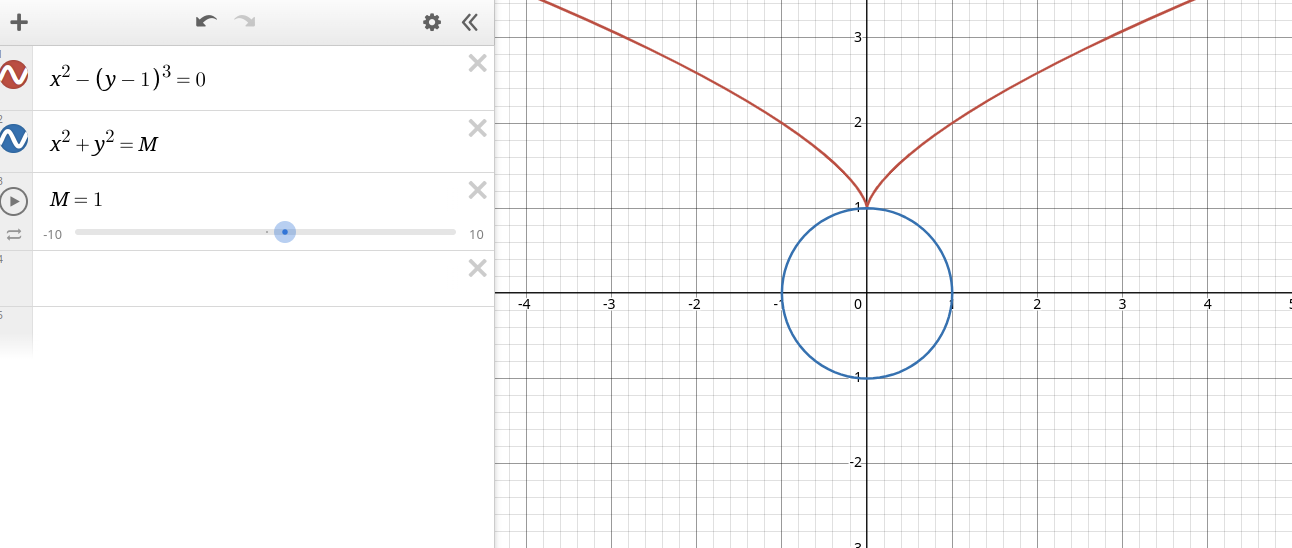
\includegraphics[width=0.85\linewidth]{figures/BT07.png}
        \caption{Miền khả thi của bài toán (\ref{problem:07}).}
        \label{fig:feasible_region_problem_03}
    \end{figure}
    \item Chứng minh rằng không tồn tại điểm nào thỏa mãn điều kiện KKT. Ta có dạng hàm Lagrangian như sau:
    \begin{equation}
        L(x, y, \mu) = x^2 + y^2 + \mu_1\left[x^2 - (y - 1)^3\right]
    \end{equation}
    và các điều kiện KKT được viết như sau:
    \begin{itemize}
        \item \begin{equation}
            \dfrac{\partial L}{\partial x} = 2x + 2\mu_1x = 0 \Leftrightarrow \begin{cases}
                x = 0\\ 
                \text{hoặc} \\
                \mu_1 = -1
            \end{cases}
        \end{equation}
        \item \begin{equation}
            \dfrac{\partial L}{\partial y} = 2y - 3\mu_1(y-1)^2 = 0
        \end{equation}
        \item \begin{equation}
            x^2 - (y - 1)^3 = 0
        \end{equation}
    \end{itemize}
    Nếu $x = 0$ thì 
    \begin{equation}
        \begin{cases}
            y = 1\\
            \mu_1 = t, t \in \R
        \end{cases}
    \end{equation} thì $(x, y) = (0,1)$ không thỏa điều kiện KKT vì không thể xác định được $\mu_1$.
    Nếu $\mu_1 = -1$ thì
    \begin{equation}
        \begin{cases}
            2y + 3(y-1)^2 = 0\\
            x^2 - (y-1)^2 = 0
        \end{cases}
    \end{equation}
    thì hệ này vô nghiệm.
    Vậy, ta không tìm được điểm KKT nào.
    \item Tìm tất cả các điểm thỏa mãn điều kiện FJ. Ta có dạng yếu của hàm Lagrangian như sau:
    \begin{equation}
        L(x, y, \lambda, \mu) = \lambda_0(x^2 + y^2) + \mu_1\left[x^2 - (y - 1)^3\right]
    \end{equation}
    và các điều kiện FJ được viết như sau:
    \begin{itemize}
        \item \begin{equation}
            \dfrac{\partial L}{\partial x} = 2\lambda_0x + 2\mu_1x = 0 \Leftrightarrow \begin{cases}
                x = 0\\ 
                \text{hoặc} \\
                \mu_1 = -\lambda_0
            \end{cases}
        \end{equation}
        \item \begin{equation}
            \dfrac{\partial L}{\partial y} = 2\lambda_0y - 3\mu_1(y-1)^2 = 0
        \end{equation}
        \item \begin{equation}
            x^2 - (y - 1)^3 = 0
        \end{equation}
    \end{itemize}
    Nếu $x = 0$ thì 
    \begin{equation}
        \begin{cases}
            y = 1\\
            \lambda_0 = 0\\
            \mu_1 = t, t \in \R
        \end{cases}
    \end{equation}
     thì hệ này có nghiệm $(x, y) = (0,1)$
     Nếu $\mu_1 = -\lambda_0$ thì
    \begin{equation}
        \begin{cases}
            2\lambda_0y - 3\lambda_0(y-1)^2 = 0\\
            x^2 - (y-1)^2 = 0
        \end{cases}
        \Leftrightarrow
        \begin{cases}
            \lambda_0 \ne 0 \\ 
            y = \dfrac{4+\sqrt{7}}{3}\quad\text{hoặc}\quad y = \dfrac{4-\sqrt{7}}{3} \\\\
            x = \sqrt{\left(\dfrac{1+\sqrt{7}}{3}\right)}\quad\text{hoặc}\quad x = -\sqrt{\left(\dfrac{1+\sqrt{7}}{3}\right)}
        \end{cases}
    \end{equation}
    Vậy các điểm FJ lần lượt là:
    \begin{equation}
        \left(\sqrt{\left(\dfrac{1+\sqrt{7}}{3}\right)}, \dfrac{4+\sqrt{7}}{3}\right); \left(-\sqrt{\left(\dfrac{1+\sqrt{7}}{3}\right)}, \dfrac{4-\sqrt{7}}{3}\right)
    \end{equation}
    \item Khi thử giải bài toán tối ưu bằng cách thế ngược $x^2 = (y - 1)^3$ trong hàm mục tiêu, do đó giảm thiểu nó về bài toán không ràng buộc:
    \begin{equation}
        \begin{aligned}
            \min \quad & y^2 + (y-1)^3\\
        \end{aligned}
    \end{equation}
    Những có điều gì đó chưa đúng với phương pháp này. Đó là gì, và làm thế nào để hiệu chỉnh lại cho đúng. 

    Ta thấy nếu $x^2 - (y - 1)^3 = 0$ thì ta phải có $y \geq 1$. Đây là một ràng buộc ẩn và nó sẽ biến mất nếu ta thay thế $x^2 = (y - 1)^2$ trong hàm mục tiêu. Nếu ta loại bỏ $x$, ta phải đảm bảo rằng $y \geq 1$. Nếu ta không thêm vào ràng buộc này, thì hàm mục tiểu $y^2 + (y-1)^3$ sẽ không bị chặn.
\end{enumerate}
\end{solution}
    \section{Bài 08}
Trong bài toán tối ưu
\begin{equation}
    \begin{aligned}
        \min \quad & (x+1)^2 + y^2\\
        \textrm{s.t.} \quad & x + y \leq 0\\
        &x^2 + y^2 = 1
    \end{aligned}
\end{equation}
bắt đầu từ những điểm khởi tạo khác nhau, một thuật toán số trả về những điểm $(x^{*}, y^{*})$ như các ứng viên cho một cực tiểu địa phương:
\begin{itemize}
    \item $\left(\dfrac{-1}{\sqrt{2}}, \dfrac{1}{\sqrt{2}}\right)$
    \item $(-1, 0)$
    \item $(0, 0)$
    \item $\left(\dfrac{-1}{{2}}, \dfrac{-\sqrt{3}}{{2}}\right)$
\end{itemize}
\begin{enumerate}[label=(\alph*)]
    \item Xác định những điểm nào trong đó mà thỏa mãn điều kiện KKT.
    \item Xác định những điểm KKT nào mà thỏa mãn điều kiện cần cấp hai.
    \item Xác định những điểm KKT nào mà thỏa mãn điều kiện đủ cấp hai.
\end{enumerate}

\begin{solution}

    Các thành phần trong bài toán này như sau:
    \begin{align}
        \begin{aligned}
            f(x,y) &= (x+1)^2 + y^2\\
            g_1(x, y) &= x + y \\
            h_1(x,y) &= x^2 + y^2 - 1\\
        \end{aligned}
    \end{align}
    Ta hình thành hàm Lagrangian như sau
    \begin{equation}
        L(x,y, \lambda) = (x+1)^2 + y^2 + \lambda_1(x + y) + \mu_1(x^2 + y^2 - 1)
    \end{equation}
    và điều kiện KKT có thể được viết như sau:
    \begin{itemize}
        \item \begin{equation}
            \dfrac{\partial L}{\partial x} = 2(x+1) + \lambda_1 + 2x\mu_1 = 0 \Leftrightarrow x = \dfrac{-\lambda_1 - 2}{2(\mu_1 + 1)}
        \end{equation}
        \item \begin{equation}
            \dfrac{\partial L}{\partial y} = 2y + \lambda_1 + 2y\mu_1 = 0 \Leftrightarrow y = \dfrac{-\lambda_1}{2(1+\mu_1)}
        \end{equation}
        \item \begin{equation}
            \lambda_1 \geq 0, x + y \leq 0, \lambda_1(x + y) = 0
        \end{equation}
        \item \begin{equation}
            x^2 + y^2 - 1 = 0
        \end{equation}
    \end{itemize}
    \begin{enumerate}[label=(\alph*)]
        \item Xác định những điểm nào trong đó mà thỏa mãn điều kiện KKT.
        \begin{itemize}
            \item Xem xét điểm $\left(\dfrac{-1}{\sqrt{2}}, \dfrac{1}{\sqrt{2}}\right)$
            \begin{equation}
                \left(\dfrac{-1}{\sqrt{2}}\right)^2 + \left(\dfrac{1}{\sqrt{2}}\right)^2 - 1 = 0
            \end{equation}
            \begin{equation}
                \lambda_1 \geq 0, \left(\dfrac{-1}{\sqrt{2}}\right) +  \left(\dfrac{1}{\sqrt{2}}\right) = 0
            \end{equation}
            \begin{equation}
                \begin{cases}
                    \dfrac{-1}{\sqrt{2}} + \dfrac{\lambda_1 + 2}{2(\mu_1 + 1)} = 0 \\
                    \dfrac{1}{\sqrt{2}} + \dfrac{\lambda_1}{2(1+\mu_1)} = 0
                \end{cases}
                \Leftrightarrow
                \begin{cases}
                    \lambda_1 = -1 \\
                    \mu_1 = \frac{\sqrt{2}}{2}-1
                \end{cases}
            \end{equation}
            Vậy điểm $\left(\dfrac{-1}{\sqrt{2}}, \dfrac{1}{\sqrt{2}}\right)$ không thỏa mãn điều kiện KKT.
            \item Xem xét điểm $(-1, 0)$
            \begin{equation}
                (-1)^2 + 0^2 - 1 = 0
            \end{equation}
            \begin{equation}
                \lambda_1 \geq 0, \lambda_1(-1 + 0) = -\lambda_1 \leq 0 \Rightarrow \lambda_1 = 0
            \end{equation}
            \begin{equation}
                \begin{cases}
                     -1 + \dfrac{\lambda_1 + 2}{2(\mu_1 + 1)} = 0 \\
                        \dfrac{\lambda_1}{2(1+\mu_1)} = 0
                \end{cases}
                \Leftrightarrow
                \begin{cases}
                    \lambda_1 = 0 \\ 
                    \mu_1 = 0
                \end{cases}
            \end{equation}
            Vậy, điểm $(-1, 0)$ thỏa mãn điều kiện KKT.
            \item Xem xét điểm $(0, 0)$
            \begin{equation}
                (0)^2 + 0^2 - 1 \ne 0
            \end{equation}
            Vậy, điểm $(0, 0)$ không thỏa mãn điều kiện KKT.
            \item Xem xét điểm $\left(\dfrac{-1}{{2}}, \dfrac{-\sqrt{3}}{{2}}\right)$
            \begin{equation}
                \left(\dfrac{-1}{{2}}\right)^2 + \left(\dfrac{-\sqrt{3}}{{2}}\right)^2 - 1 = 0
            \end{equation}
            \begin{equation}
                \lambda_1 \geq 0, \lambda_1(\dfrac{-1}{{2}} + \dfrac{-\sqrt{3}}{{2}}) \leq 0 \Rightarrow \lambda_1 = 0 \Rightarrow y = 0
            \end{equation}
            Vây điểm $\left(\dfrac{-1}{{2}}, \dfrac{-\sqrt{3}}{{2}}\right)$ không thỏa mãn điều kiện KKT.
        \end{itemize}
        \item Xác định những điểm KKT nào mà thỏa mãn điều kiện cần cấp hai.
        \item Xác định những điểm KKT nào mà thỏa mãn điều kiện đủ cấp hai.
    \end{enumerate}
\end{solution}
    \section{Bài 09}
Xem xét bài toán cực đại
\begin{equation}
    \label{problem:09}
    \begin{aligned}
        \max \quad & x^2 + y\\
        \textrm{s.t.} \quad & x^2 + y^2 \leq 9,\\
        &x + y \leq 1.
    \end{aligned}
\end{equation}
\begin{enumerate}[label=(\alph*)]
    \item Vẽ miền khả thi và đường mức của hàm mục tiêu. Dựa trên đó, đoán cực đại toàn cục.
    \item Lập luận tại sao KKT phải thỏa mãn tại các cực đại toàn cục.
    \item Viết các điều kiện KKT, và sử dụng chúng để xác định tất cả các điểm KKT.
    \item Xác định những điểm KKT thỏa mãn điều kiện cấp hai (cần và đủ).
\end{enumerate}

\begin{solution}

    Các thành phần trong bài toán này như sau:
    \begin{align}
        \begin{aligned}
            f(x,y) &= x^2 + y\\
            g_1(x, y) &= x^2 + y^2 - 9 \\
            g_2(x, y) &= x + y  - 1 \\
        \end{aligned}
    \end{align}
    \begin{enumerate}[label=(\alph*)]
        \item Vẽ miền khả thi và đường mức của hàm mục tiêu. Dựa trên đó, đoán cực đại toàn cục.
        \begin{figure}[h!]
            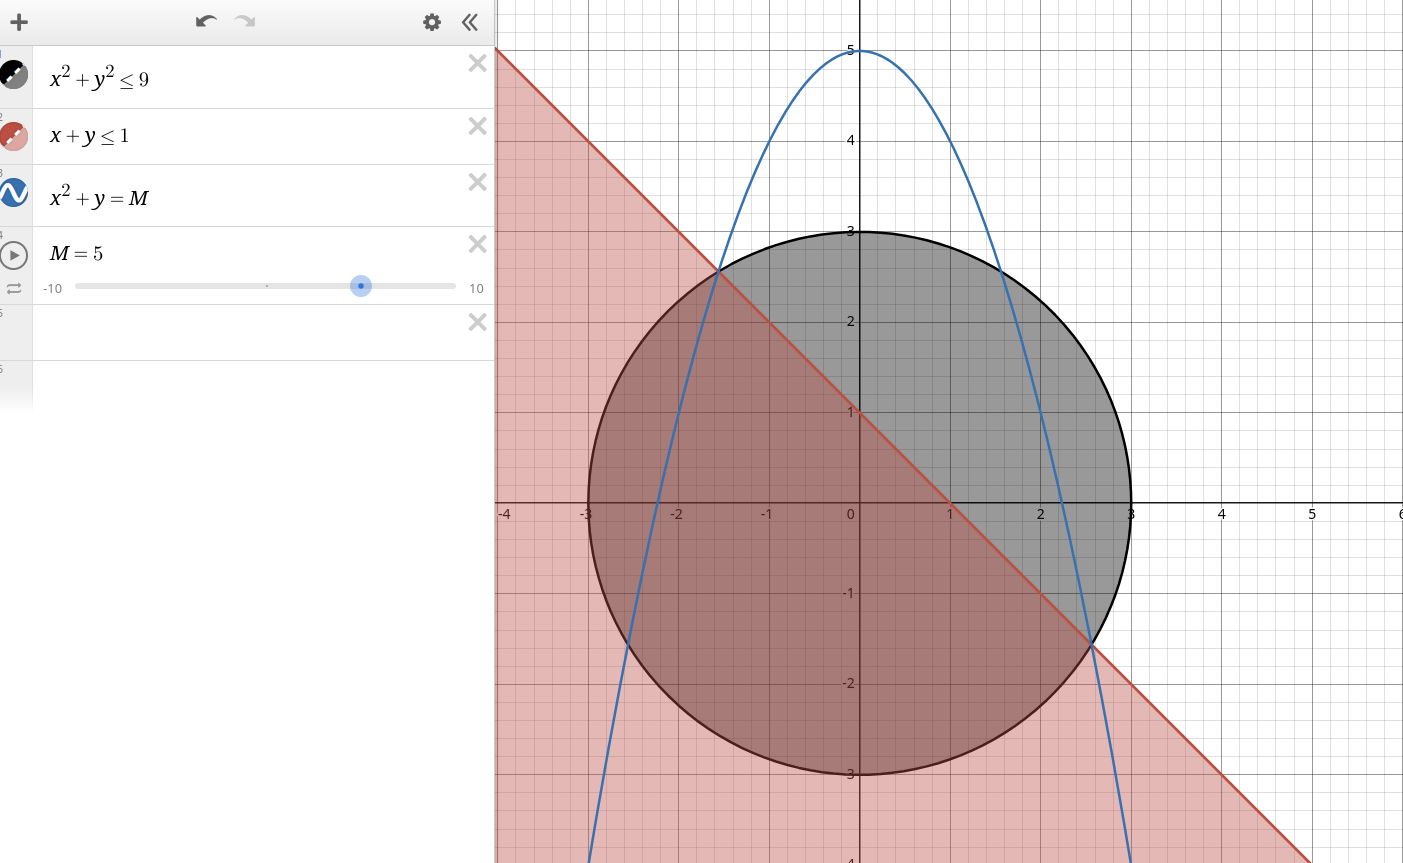
\includegraphics[width=0.85\linewidth]{figures/BT09.png}
            \caption{Miền khả thi của bài toán (\ref{problem:09}).}
            \label{fig:feasible_region_problem_09}
        \end{figure}
        Ta có thể vẽ được miền khả thi và đường múc của hàm mục tiêu như Hình (\ref{fig:feasible_region_problem_09}). Dựa trên hình vẽ, ta có thể đoán được các cực trị của bài toán nằm tại giao điểm giữa các phương trình $f(x,y), g_1(x, y)$ và $g_2(x, y)$. Điểm cực đại sẽ là giao điểm phía trên.
        \item Lập luận tại sao KKT phải thỏa mãn tại các cực đại toàn cục. Ta nhận thấy, bài toán này có cực đại toàn cục bởi vì miền ràng buộc là compact. Ta có đạo hàm của các ràng buộc lần lượt là 
        \begin{itemize}
            \item $\Delta g_1(x, y) = 2(x,y)$ 
            \item $\Delta g_2(x,y) = (1,1)$
        \end{itemize}
        Dễ dàng thấy rằng, đạo hàm thứ hai luôn luôn khác không, và đạo hàm thứ nhất chỉ bằng không tại gốc tọa độ nơi mà không thoả mãn ràng buộc $g1$ không kích hoạt. Do đó, các điều kiện KKT phải được thỏa mãn tại bất kỳ cực tiểu cục bộ $(x^{*}, y^{*})$ nào mà có ít nhất một ràng buộc được kích hoạt. Nếu cả hai ràng buộc được kích hoạt, các đẳng thức $x^{2} + y^{2} = 9$ và $x + y = 1$ cho nghiệm 
        \begin{equation}
            y = \dfrac{1+\sqrt{17}}{2}\quad\text{hoặc}\quad y = \dfrac{1-\sqrt{17}}{2}
        \end{equation}
        và các đạo hàm $\{\Delta g_1(x, y), \Delta g_2(x, y) \}$ độc lập tuyến tính. Do đó, các điều kiện KKT phải thỏa ở ất cả các điểm KKT có thể có.
        \item Viết các điều kiện KKT, và sử dụng chúng để xác định tất cả các điểm KKT. Ta có dạng của hàm Lagrangian như sau:
        \begin{equation}
            L(x,y,\lambda) = x^2 + y + \lambda_1(x^2 + y^2 - 9) + \lambda_2(x + y  - 1)
        \end{equation}
        và các điều kiện KKT được viết như sau:
        \begin{itemize}
            \item \begin{equation}
                \dfrac{\partial L}{\partial x} = 2x + 2\lambda_1x + \lambda_2 = 0 \Leftrightarrow x = -\dfrac{\lambda_2}{2+2\lambda_1}
            \end{equation}
            \item \begin{equation}
                \dfrac{\partial L}{\partial y} = 1 + 2\lambda_1y + \lambda_2 = 0 \Leftrightarrow y = -\dfrac{\lambda_2 + 1}{2\lambda_1}
            \end{equation}
            \item \begin{equation}
                \lambda_1 \geq 0, x^2 + y^2 - 9 \leq 0, \lambda_1(x^2 + y^2 - 9) = 0
            \end{equation}
            \item \begin{equation}
                \lambda_2 \geq 0, x + y  - 1 \leq 0, \lambda_2(x + y  - 1) = 0
            \end{equation}
        \end{itemize}
        Ta xem xét những trường hợp có thể có cho dấu của các nhân tử
        \begin{itemize}
            \item Trường hợp 1 ($\lambda_1 > 0, \lambda_2 > 0)$, ta có hệ
            \begin{equation}
                \begin{cases}
                    x^2 + y^2 - 9 = 0\\
                    x + y  - 1 = 0\\
                \end{cases}
                \Leftrightarrow
                \begin{cases}
                    x = \dfrac{1-\sqrt{17}}{2}\\
                    y = \dfrac{1+\sqrt{17}}{2}
                \end{cases}
                \quad
                \text{hoặc}
                \begin{cases}
                    x = \dfrac{1+\sqrt{17}}{2}\\
                    y = \dfrac{1-\sqrt{17}}{2}
                \end{cases}
            \end{equation}
            Cả hai điểm này đều thỏa mãn ràng buộc nên chúng là các điểm KKT.
            \item Trường hợp 2 ($\lambda_1 = 0, \lambda_2 > 0)$, ta không thể giải được do không xác định cho phương trình (9.6)
            \item Trường hợp 3 ($\lambda_1 > 0, \lambda_2 = 0)$, ta có
            \begin{equation}
                \begin{cases}
                    x = 0\\
                    y = -\frac{1}{2\lambda_1}
                    x^2 + y^2 - 9 = 0\\
                \end{cases}
                \Leftrightarrow
                \begin{cases}
                    x = 0\\
                    \lambda_1 = \pm\dfrac{1}{6}\\
                    y = \pm 3
                \end{cases}
            \end{equation}
            Trong đó $(x, y) = (0, -3)$ thỏa mãn ràng buộc, do đó điểm này là một điểm KKT.
            \item Trường hợp 4 ($\lambda_1 = 0, \lambda_2 = 0)$, ta không thể giải được do không xác định cho phương trình (9.6)
        \end{itemize}
        \item Xác định những điểm KKT thỏa mãn điều kiện cấp hai (cần và đủ).
    \end{enumerate}
\end{solution}
     \section{Bài 10}

Xem xét bài toán
\begin{equation}
    \begin{aligned}
        \max \quad & x_1^3 + x_2^3 + \dots + x_n^3\\
        \textrm{s.t.} \quad & x_1^2 + x_2^2 + \dots + x_n^2 = 1,\\
    \end{aligned}
\end{equation}
\begin{enumerate}[label=(\alph*)]
    \item Chứng minh rằng điều kiện KKT phải thỏa mãn tại mỗi cực đại cục bộ.
    \item Xác định tất cả các điểm KKT.
    \item Xác định các cực đại toàn cục của bài toán.
    \item Sử dụng câu trên để chứng minh bất đẳng thức
    \begin{equation}
        \sum_{i=1}^n| x_i|^3 \leq \left(\sum_{i=1}^nx_i^2\right)^{\frac{3}{2}}, \forall (x_1, \dots, x_n) \in \R^n
    \end{equation}
    \item Nếu có những KKT khác những cực tiểu cục bộ, xác định một trong các cực đại cục bộ.
\end{enumerate}


\begin{solution}

    Các thành phần trong bài toán này như sau:
    \begin{align}
        \begin{aligned}
            f(x) &= x_1^3 + x_2^3 + \dots + x_n^3 = \sum_{j=1}^nx_j^3\\
            h_1(x) &= x_1^2 + x_2^2 + \dots + x_n^2 - 1 = -1 + \sum_{j=1}^nx_j^2  \\
        \end{aligned}
    \end{align}
    \begin{enumerate}[label=(\alph*)]
        \item Chứng minh rằng điều kiện KKT phải thỏa mãn tại mỗi cực đại cục bộ. Ta dễ dàng thấy được miền khả thi là compact, do đó theo định lý Weierstrass, bài toán này có cực đại toàn cục và cực đại toàn cục. 
        \item Xác định tất cả các điểm KKT. Ta viết hàm Lagrangian như sau:
        \begin{equation}
            L(x, \mu) = \sum_{j=1}^nx_j^3 + \dfrac{\mu_1}{2}\left(-1 + \sum_{j=1}^nx_j^2\right)
        \end{equation}
        và các điều kiện KKT
        \begin{itemize}
            \item \begin{equation}
                \dfrac{\partial L}{\partial x_i} = 3x_i^2 + 2\dfrac{\mu_1}{2} x_i = 3x_i^2 + \mu_1x_i = 0
            \end{equation}
            \item \begin{equation}
                -1 + \sum_{i=1}^nx_i^2 = 0
            \end{equation}
        \end{itemize}
        Tính tổng theo điều kiện KKT thứ nhất
        \begin{equation}
            3\sum_{i=1}^nx_i^2 + \mu_1\left(\sum_{i=1}^nx_i\right) = 3 + \mu_1\left(\sum_{i=1}^nx_i\right) = 0 \Leftrightarrow \left(\sum_{i=1}^nx_i\right) = -\dfrac{3}{\mu_1}
        \end{equation}
        Và bởi vì tất cả các hàm trong bài toán tối ưu là đối xứng với các biến $x_i$, không mất tính tổng quát, ta có thể giả định rằng 
        \begin{equation}
            x := (x_1, \dots, x_n) = (\underset{k\text{ lần}}{\underbrace{x_{+}, \dots, x_{+}}},\underset{n-k\text{ lần}}{\underbrace{x_{-}, \dots, x_{-}}})
        \end{equation}
        Từ biểu thức (10.8)
        \begin{equation}
            kx_{+}+(n-k)x_{-} = -\dfrac{3}{\mu_1} \Leftrightarrow x_{-} = -\dfrac{\dfrac{3}{\mu_1}+kx_{+}}{n-k}
        \end{equation}
        Điều kiện KKT thứ hai trở thành
        \begin{equation}
            kx_{+}^2 + (n-k)x_{-}^2 = 1 \Leftrightarrow nkx_{+}^2 +\dfrac{6k}{\mu_1}x_{+} + \dfrac{9}{\mu_1} = 0
        \end{equation}
        Ta có:
        \begin{equation}
            \Delta = 36\left(\dfrac{k^2}{\mu_1^2}-\dfrac{nk}{\mu_1}\right)
        \end{equation}
        Để phương trình (10.10) có nghiệm, thì $\Delta \geq 0 \Leftrightarrow k \geq n\mu_1$ có nghĩa là $0\leq \mu_1 \leq 1$. Ta có thể viết công thức nghiệm cho $x_{+}$ như sau:
        \begin{equation}
            x_{+} = \dfrac{-\dfrac{6k}{\mu_1}\pm 6\sqrt{\dfrac{k^2}{\mu_1^2}-\dfrac{nk}{\mu_1}}}{2nk}
        \end{equation}
        Thay vào biểu thức (10.9), ta được
        \begin{equation}
            x_{-} = -\dfrac{\dfrac{3}{\mu_1} + \dfrac{-\dfrac{6k}{\mu_1}\pm 6\sqrt{\dfrac{k^2}{\mu_1^2}-\dfrac{nk}{\mu_1}}}{2n}}{n-k}
        \end{equation}
        \item Xác định các cực đại toàn cục của bài toán. Như chứn minh trên, ta được các nghiệm
        \begin{equation}
            x_{+} = \dfrac{-\dfrac{6k}{\mu_1}\pm 6\sqrt{\dfrac{k^2}{\mu_1^2}-\dfrac{nk}{\mu_1}}}{2nk};\quad x_{-} = -\dfrac{\dfrac{3}{\mu_1} + \dfrac{-\dfrac{6k}{\mu_1}\pm 6\sqrt{\dfrac{k^2}{\mu_1^2}-\dfrac{nk}{\mu_1}}}{2n}}{n-k}
        \end{equation}
        Cực đại toàn cục đạt được khi $k=n-1, \mu_1 = 1$, 
        \begin{equation}
            x_{+} = -\dfrac{6}{2n}
        \end{equation}
        \item Sử dụng câu trên để chứng minh bất đẳng thức
        \begin{equation}
            \sum_{i=1}^n| x_i|^3 \leq \left(\sum_{i=1}^nx_i^2\right)^{\frac{3}{2}}, \forall (x_1, \dots, x_n) \in \R^n
        \end{equation}
        \item Nếu có những KKT khác những cực tiểu cục bộ, xác định một trong các cực đại cục bộ.
    \end{enumerate}
\end{solution}

    \section{Bài 11}

Xem xét bài toán biến thể
\begin{equation}
    \begin{aligned}
        \max \quad & x_1^3 + x_2^3 + \dots + x_n^3\\
        \textrm{s.t.} \quad & x_1^4 + x_2^4 + \dots + x_n^4 = 1,\\
    \end{aligned}
\end{equation}
Trả lời các câu hỏi tương ứng như Bài 10, và điều chỉnh và chứng minh dạng đúng của bất đẳng thức (c).

\begin{solution}

    Các thành phần trong bài toán này như sau:
    \begin{align}
        \begin{aligned}
            f(x) &= x_1^3 + x_2^3 + \dots + x_n^3 = \sum_{j=1}^nx_j^3\\
            h_1(x) &= x_1^4 + x_2^4 + \dots + x_n^4 - 1 = -1 + \sum_{j=1}^nx_j^4  \\
        \end{aligned}
    \end{align}

    Ta dễ dàng thấy được miền khả thi là compact, do đó theo định lý Weierstrass, bài toán này có cực đại toàn cục và cực đại toàn cục. 

     Xác định tất cả các điểm KKT. Ta viết hàm Lagrangian như sau:
        \begin{equation}
            L(x, \mu) = \sum_{j=1}^nx_j^3 + \dfrac{\mu_1}{4}\left(-1 + \sum_{j=1}^nx_j^4\right)
        \end{equation}
        và các điều kiện KKT
        \begin{itemize}
            \item \begin{equation}
                \dfrac{\partial L}{\partial x_i} = 3x_i^2 + 4\dfrac{\mu_1}{4} x_i^3 = 3x_i^2 + \mu_1x_i^3 = x_i^2(3+\mu_1x_i) = 0 \Leftrightarrow \begin{cases}
                    x_i = 0\quad\text{(loại)}\\
                    x_i = -\dfrac{3}{\mu_1}
                \end{cases}
            \end{equation}
            \item \begin{equation}
                \sum_{i=1}^nx_i^4 = 1 \Leftrightarrow \sum_{i=1}^nx_i^2 = 1 
            \end{equation}
        \end{itemize}
    Tính tổng theo điều kiện KKT thứ nhất
        \begin{equation}
            3\sum_{i=1}^nx_i^2 + \mu_1\left(\sum_{i=1}^nx_i\right) = 3 + \mu_1\left(\sum_{i=1}^nx_i\right) = 0 \Leftrightarrow \left(\sum_{i=1}^nx_i\right) = -\dfrac{3}{\mu_1}
        \end{equation}
        Và bởi vì tất cả các hàm trong bài toán tối ưu là đối xứng với các biến $x_i$, không mất tính tổng quát, ta có thể giả định rằng 
        \begin{equation}
            x := (x_1, \dots, x_n) = (\underset{k\text{ lần}}{\underbrace{x_{+}, \dots, x_{+}}},\underset{n-k\text{ lần}}{\underbrace{x_{-}, \dots, x_{-}}})
        \end{equation}
        Từ biểu thức (11.8)
        \begin{equation}
            kx_{+}+(n-k)x_{-} = -\dfrac{3}{\mu_1} \Leftrightarrow x_{-} = -\dfrac{\dfrac{3}{\mu_1}+kx_{+}}{n-k}
        \end{equation}
        Điều kiện KKT thứ hai trở thành
        \begin{equation}
            kx_{+}^2 + (n-k)x_{-}^2 = 1 \Leftrightarrow nkx_{+}^2 +\dfrac{6k}{\mu_1}x_{+} + \dfrac{9}{\mu_1} = 0
        \end{equation}
        Ta có:
        \begin{equation}
            \Delta = 36\left(\dfrac{k^2}{\mu_1^2}-\dfrac{nk}{\mu_1}\right)
        \end{equation}
        Để phương trình (11.10) có nghiệm, thì $\Delta \geq 0 \Leftrightarrow k \geq n\mu_1$ có nghĩa là $0\leq \mu_1 \leq 1$. Ta có thể viết công thức nghiệm cho $x_{+}$ như sau:
        \begin{equation}
            x_{+} = \dfrac{-\dfrac{6k}{\mu_1}\pm 6\sqrt{\dfrac{k^2}{\mu_1^2}-\dfrac{nk}{\mu_1}}}{2nk}
        \end{equation}
        Thay vào biểu thức (11.9), ta được
        \begin{equation}
            x_{-} = -\dfrac{\dfrac{3}{\mu_1} + \dfrac{-\dfrac{6k}{\mu_1}\pm 6\sqrt{\dfrac{k^2}{\mu_1^2}-\dfrac{nk}{\mu_1}}}{2n}}{n-k}
        \end{equation}
        \item Xác định các cực đại toàn cục của bài toán. Như chứn minh trên, ta được các nghiệm
        \begin{equation}
            x_{+} = \dfrac{-\dfrac{6k}{\mu_1}\pm 6\sqrt{\dfrac{k^2}{\mu_1^2}-\dfrac{nk}{\mu_1}}}{2nk};\quad x_{-} = -\dfrac{\dfrac{3}{\mu_1} + \dfrac{-\dfrac{6k}{\mu_1}\pm 6\sqrt{\dfrac{k^2}{\mu_1^2}-\dfrac{nk}{\mu_1}}}{2n}}{n-k}
        \end{equation}
        Cực đại toàn cục đạt được khi $k=n-1, \mu_1 = 1$, 
        \begin{equation}
            x_{+} = -\dfrac{6}{2n}
        \end{equation}
\end{solution}
    \section{Bài 12}

Xem xét bài toán tối ưu bậc hai có ràng buộc
\begin{equation}
    \begin{aligned}
        \min \quad & q(x) = \dfrac{1}{2}\left \langle Qx,x \right \rangle + \left \langle c,x \right \rangle\\
        \textrm{s.t.} \quad & Ax = b,\\
    \end{aligned}
\end{equation}
có một ma trận đối xứng $Q$ kích thước $n \times n$, và một vector $c \in \R^n$.
\begin{enumerate}[label=(\alph*)]
    \item Chứng minh rằng một cực tiểu địa phương $x^*$ phải thỏa mãn các điều kiện KKT $Qx^* + c \in R(A^T)$ và $Ax^* = b$.
    \item Chứng minh một cực tiểu địa phương $x^*$ phải thỏa mãn điều kiện đủ bậc hai rằng $Q$ bán xác dịnh dương trong không gian con (subspace) $N(A)$, không gian không (null space) của $A$.
    \item Chứng minh rằng một điểm KKT 
\end{enumerate}

\begin{solution}

    Ta nhận thấy hàm ràng buộc có đạo hàm khác không tại mọi điểm trong miền khả thi, ta có thể giả sử rằng $\lambda_0 = 1$. Bằng cách bình phương hai vế của phương trình hàm ràng buộc, ta có thể viết lại bài toán như sau:
    \begin{equation}
        \begin{aligned}
            \min \quad & q(x) = \dfrac{1}{2}\left \langle Qx,x \right \rangle + \left \langle c,x \right \rangle\\
            \textrm{s.t.} \quad & \left \| x \right \|^2 = A^{-2}b^2,\\
        \end{aligned}
    \end{equation}
    và hàm Lagrangian được viết như sau:
    \begin{equation}
        L = \dfrac{1}{2}\left \langle Qx,x \right \rangle + \left \langle c,x \right \rangle + \dfrac{\lambda}{2}\left(\left \| x \right \|^2 - A^{-2}b^2\right)
    \end{equation}
    Tại một cực tiểu địa phương $x^*$ của bài toán, ta có các điều kiện KKT như sau:
    \begin{enumerate}[label=(\alph*)]
        \item $\Delta_x L = (Q+\lambda I)x^* + c = 0$, tức là $Qx^* + c \in R(A^T)$.
        \item $\lambda \geq, \left \| x^* \right \| \leq A^{-1}b, \lambda(\left \| x^* \right \| - A^{-1}b) = 0$, tức là $Ax^* = b$.
    \end{enumerate}
    Từ điều kiện (a) và (b), cùng với điều kiện bậc hai, ta nhận thấy $Q + \lambda I$ là ma trận bán xác định dương. Thật vậy, trước hết ta giả định rằng $x^*$ là một cực tiểu địa phương của bài toán. Nếu $\left \| x^* \right \| < A^{-1}b$, thì $\lambda = 0$ và $x^*$ là một cực tiểu địa phương không ràng buộc của $q$, và do đó $Q$ là bán xác định dương theo Định lý Weierstrass. Nếu $\left \| x^* \right \| = A^{-1}b$ và $\left \| x \right \| = A^{-1}b$ là bất kỳ điểm khả thi nào, thì $q(x) - q(x^*) \geq 0$, và
    \begin{align}
        \begin{aligned}
            &q(x) - q(x^*) \\ 
            &=\left \langle \Delta q(x^*), x - x^*\right \rangle + \dfrac{1}{2}\left \langle Q(x-x^*),  x - x^*\right \rangle \\
            &=-\lambda\left \langle  x^*, x - x^*\right \rangle + \dfrac{1}{2}\left \langle Q(x-x^*),  x - x^*\right \rangle \\
            &=  \dfrac{1}{2}\left \langle (Q+\lambda I)(x-x^*),  x - x^*\right \rangle - \dfrac{\lambda}{2}(\left \| x - x^* \right \|^2 + 2\left \langle  x^*, x - x^*\right \rangle)\\
            &= \dfrac{1}{2}\left \langle (Q+\lambda I)(x-x^*),  x - x^*\right \rangle  + \dfrac{\lambda}{2}(\left \| x \right \|^2 - \left \| x^* \right \|^2)
        \end{aligned}
    \end{align}
    Điều này chỉ ra rằng $\left \langle (Q+\lambda I)(x-x^*),  x - x^*\right \rangle \geq 0$ với mọi $\left \| x \right \| = A^{-1}b$. Bởi vì $\left \langle  x^*, x - x^*\right \rangle \leq 0$, ta có $\left \langle (Q+\lambda I)d, d \right \rangle \geq 0$ với mọi $d$ thỏa mãn $\left \langle x^*,d \right \rangle \leq 0$, do đó với mọi $d \in \R^n$, $Q + \lambda I$ là bán xác định dương.

    Hệ quả là, giả định rằng các điều kiện (a)-(c) thỏa mãn. Nếu $\left \| x^* \right \| < A^{-1}b$, thì $\lambda = 0$, và biến đổi trên chứng tỏ $x^*$ là một cực tiểu địa phương của $q$ trên $\R^n$. Nếu Nếu $\left \| x^* \right \| = A^{-1}b$, $x^*$ là một cực tiểu địa phương của $q$ trên bao đóng $\Bar{B}(0, A^{-1}b)$.
\end{solution}
\end{document}